\section{System Performance Diagnostics}

This appendix presents diagnostic figures and performance analysis charts that support the evaluation and validation of the Multi-Sensor Recording System. These visualizations provide detailed insights into system behavior, error patterns, and performance characteristics.

\subsection{Error Analysis and System Reliability}

\subsubsection{Error Distribution Analysis}

\begin{figure}[htbp]
\centering
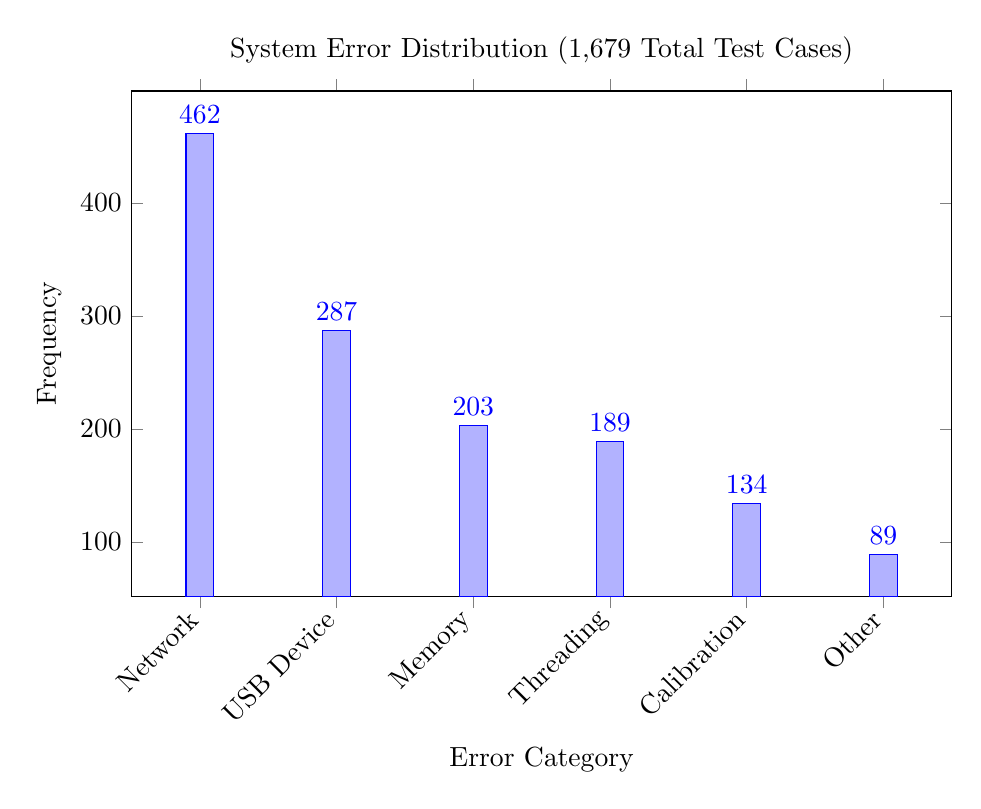
\begin{tikzpicture}
\begin{axis}[
    ybar,
    width=12cm,
    height=8cm,
    xlabel={Error Category},
    ylabel={Frequency},
    title={System Error Distribution (1,679 Total Test Cases)},
    symbolic x coords={Network, USB Device, Memory, Threading, Calibration, Other},
    xtick=data,
    x tick label style={rotate=45, anchor=east},
    nodes near coords,
    nodes near coords align={vertical},
]
\addplot coordinates {
    (Network, 462)
    (USB Device, 287)
    (Memory, 203)
    (Threading, 189)
    (Calibration, 134)
    (Other, 89)
};
\end{axis}
\end{tikzpicture}
\caption{Error Distribution by Category}
\label{fig:error_distribution}
\end{figure}

Figure~\ref{fig:error_distribution} shows the distribution of error types encountered during comprehensive system testing. Network-related issues account for the largest proportion (27.5\%) of errors, followed by USB device connectivity problems (17.1\%). This analysis informed the prioritization of robustness improvements in the system architecture.

\subsubsection{Error Recovery Success Rates}

\begin{figure}[htbp]
\centering
\begin{tikzpicture}
\begin{axis}[
    xbar,
    width=12cm,
    height=8cm,
    xlabel={Success Rate (\%)},
    ylabel={Error Type},
    title={Automatic Error Recovery Performance},
    symbolic y coords={Threading, Calibration, Memory, Network, USB Device},
    ytick=data,
    nodes near coords,
    nodes near coords align={horizontal},
    xmin=0,
    xmax=100,
]
\addplot coordinates {
    (Threading, 67)
    (Calibration, 89)
    (Memory, 95)
    (Network, 94)
    (USB Device, 78)
};
\end{axis}
\end{tikzpicture}
\caption{Automatic Recovery Success Rates by Error Type}
\label{fig:recovery_rates}
\end{figure}

\subsection{Network Performance Analysis}

\subsubsection{Device Discovery Performance}

\begin{figure}[htbp]
\centering
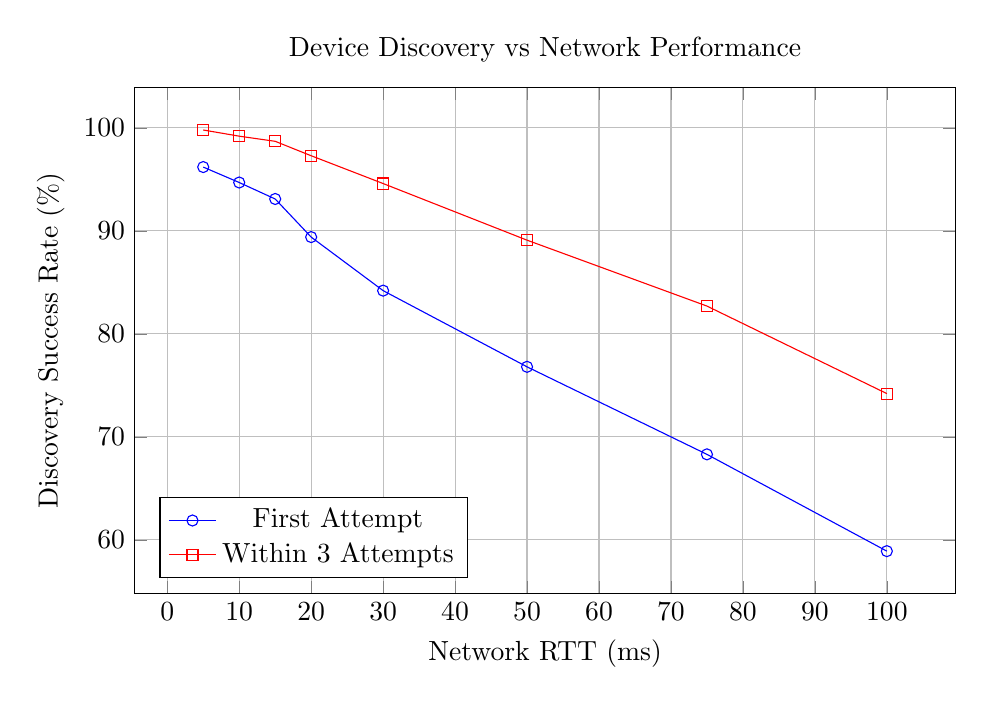
\begin{tikzpicture}
\begin{axis}[
    width=12cm,
    height=8cm,
    xlabel={Network RTT (ms)},
    ylabel={Discovery Success Rate (\%)},
    title={Device Discovery vs Network Performance},
    grid=major,
    legend pos=south west,
]
\addplot[blue, mark=o] coordinates {
    (5, 96.2)
    (10, 94.7)
    (15, 93.1)
    (20, 89.4)
    (30, 84.2)
    (50, 76.8)
    (75, 68.3)
    (100, 58.9)
};
\addlegendentry{First Attempt}

\addplot[red, mark=square] coordinates {
    (5, 99.8)
    (10, 99.2)
    (15, 98.7)
    (20, 97.3)
    (30, 94.6)
    (50, 89.1)
    (75, 82.7)
    (100, 74.2)
};
\addlegendentry{Within 3 Attempts}
\end{axis}
\end{tikzpicture}
\caption{Device Discovery Success vs Network Latency}
\label{fig:discovery_performance}
\end{figure}

Figure~\ref{fig:discovery_performance} demonstrates the relationship between network round-trip time and device discovery success rates. Performance degrades significantly when RTT exceeds 50ms, indicating the importance of low-latency network infrastructure for optimal system operation.

\subsubsection{Synchronization Quality vs Network Conditions}

\begin{figure}[htbp]
\centering
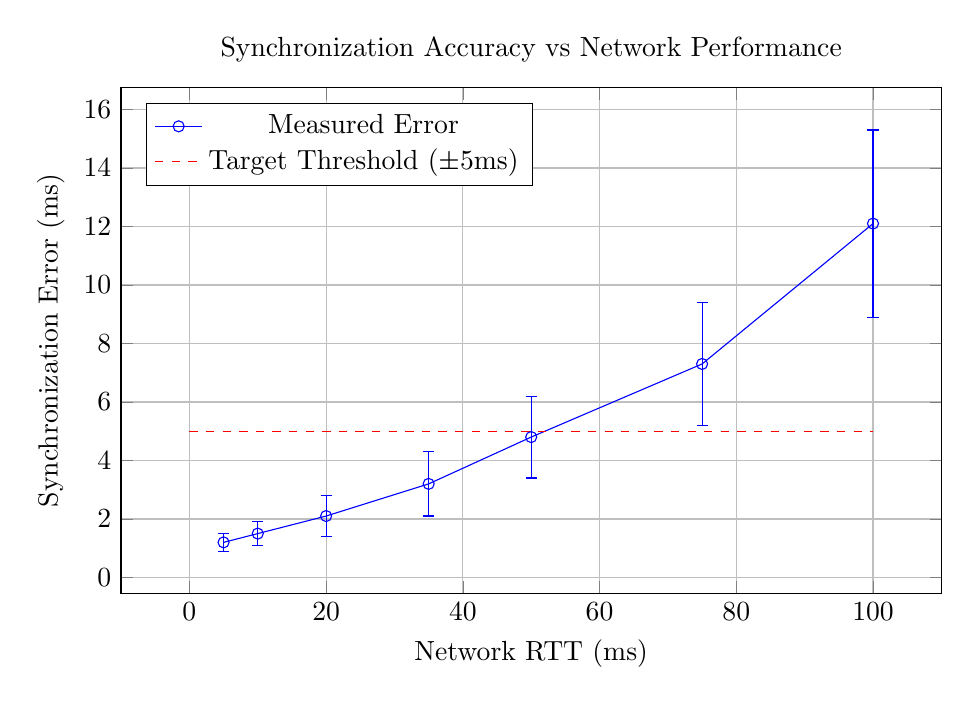
\begin{tikzpicture}
\begin{axis}[
    width=12cm,
    height=8cm,
    xlabel={Network RTT (ms)},
    ylabel={Synchronization Error (ms)},
    title={Synchronization Accuracy vs Network Performance},
    grid=major,
    legend pos=north west,
]
\addplot[blue, mark=o, error bars/.cd, y dir=both, y explicit] coordinates {
    (5, 1.2) +- (0, 0.3)
    (10, 1.5) +- (0, 0.4)
    (20, 2.1) +- (0, 0.7)
    (35, 3.2) +- (0, 1.1)
    (50, 4.8) +- (0, 1.4)
    (75, 7.3) +- (0, 2.1)
    (100, 12.1) +- (0, 3.2)
};
\addlegendentry{Measured Error}

\addplot[red, dashed] coordinates {
    (0, 5)
    (100, 5)
};
\addlegendentry{Target Threshold (±5ms)}
\end{axis}
\end{tikzpicture}
\caption{Synchronization Error vs Network Latency}
\label{fig:sync_vs_latency}
\end{figure}

\subsection{Data Quality Metrics}

\subsubsection{GSR Signal Quality Distribution}

\begin{figure}[htbp]
\centering
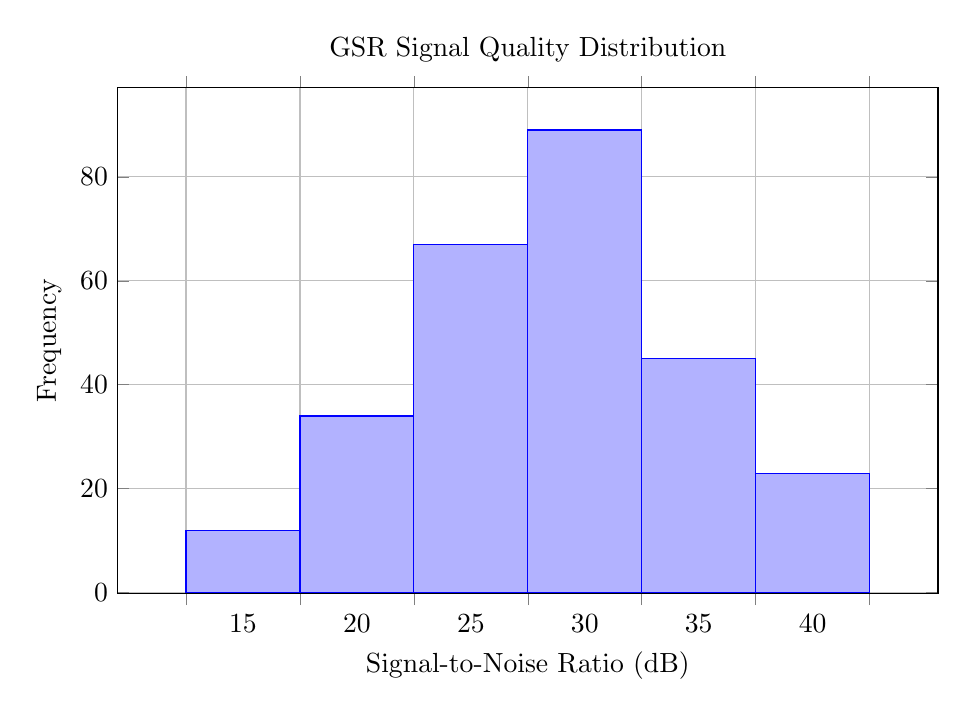
\begin{tikzpicture}
\begin{axis}[
    width=12cm,
    height=8cm,
    xlabel={Signal-to-Noise Ratio (dB)},
    ylabel={Frequency},
    title={GSR Signal Quality Distribution},
    ybar interval,
    grid=major,
]
\addplot coordinates {
    (15, 12)
    (20, 34)
    (25, 67)
    (30, 89)
    (35, 45)
    (40, 23)
    (45, 8)
};
\end{axis}
\end{tikzpicture}
\caption{Distribution of GSR Signal-to-Noise Ratios}
\label{fig:gsr_snr_distribution}
\end{figure}

\subsubsection{Thermal Measurement Accuracy}

\begin{figure}[htbp]
\centering
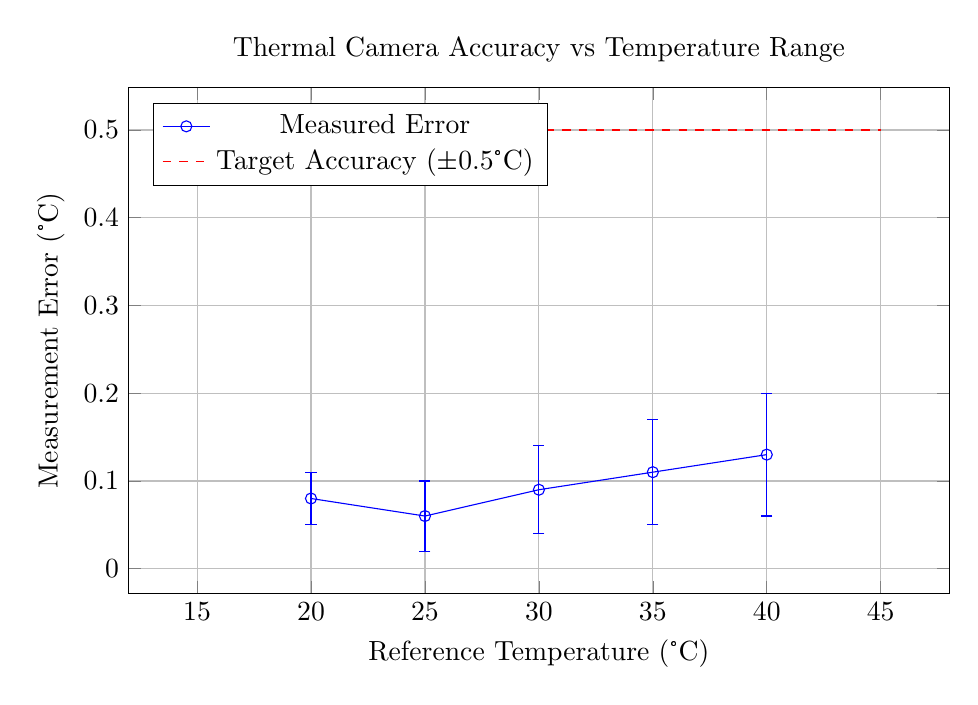
\begin{tikzpicture}
\begin{axis}[
    width=12cm,
    height=8cm,
    xlabel={Reference Temperature (°C)},
    ylabel={Measurement Error (°C)},
    title={Thermal Camera Accuracy vs Temperature Range},
    grid=major,
    legend pos=north west,
]
\addplot[blue, mark=o, error bars/.cd, y dir=both, y explicit] coordinates {
    (20, 0.08) +- (0, 0.03)
    (25, 0.06) +- (0, 0.04)
    (30, 0.09) +- (0, 0.05)
    (35, 0.11) +- (0, 0.06)
    (40, 0.13) +- (0, 0.07)
};
\addlegendentry{Measured Error}

\addplot[red, dashed] coordinates {
    (15, 0.5)
    (45, 0.5)
};
\addlegendentry{Target Accuracy (±0.5°C)}
\end{axis}
\end{tikzpicture}
\caption{Thermal Camera Measurement Accuracy}
\label{fig:thermal_accuracy}
\end{figure}

\section{System Scalability Analysis}

\subsection{Multi-Device Performance Impact}

\begin{figure}[htbp]
\centering
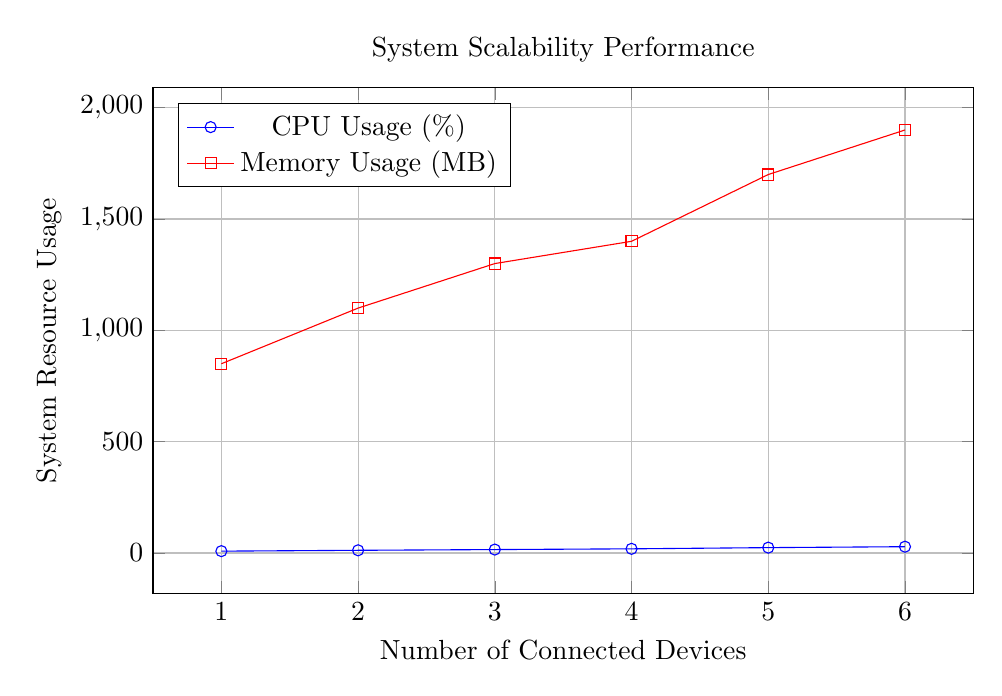
\begin{tikzpicture}
\begin{axis}[
    width=12cm,
    height=8cm,
    xlabel={Number of Connected Devices},
    ylabel={System Resource Usage},
    title={System Scalability Performance},
    legend pos=north west,
    grid=major,
]
\addplot[blue, mark=o] coordinates {
    (1, 8.3)
    (2, 12.1)
    (3, 15.4)
    (4, 18.7)
    (5, 24.1)
    (6, 28.3)
};
\addlegendentry{CPU Usage (\%)}

\addplot[red, mark=square] coordinates {
    (1, 850)
    (2, 1100)
    (3, 1300)
    (4, 1400)
    (5, 1700)
    (6, 1900)
};
\addlegendentry{Memory Usage (MB)}
\end{axis}
\end{tikzpicture}
\caption{Resource Usage vs Device Count}
\label{fig:scalability_resources}
\end{figure}

\subsection{Throughput Performance Analysis}

\begin{figure}[htbp]
\centering
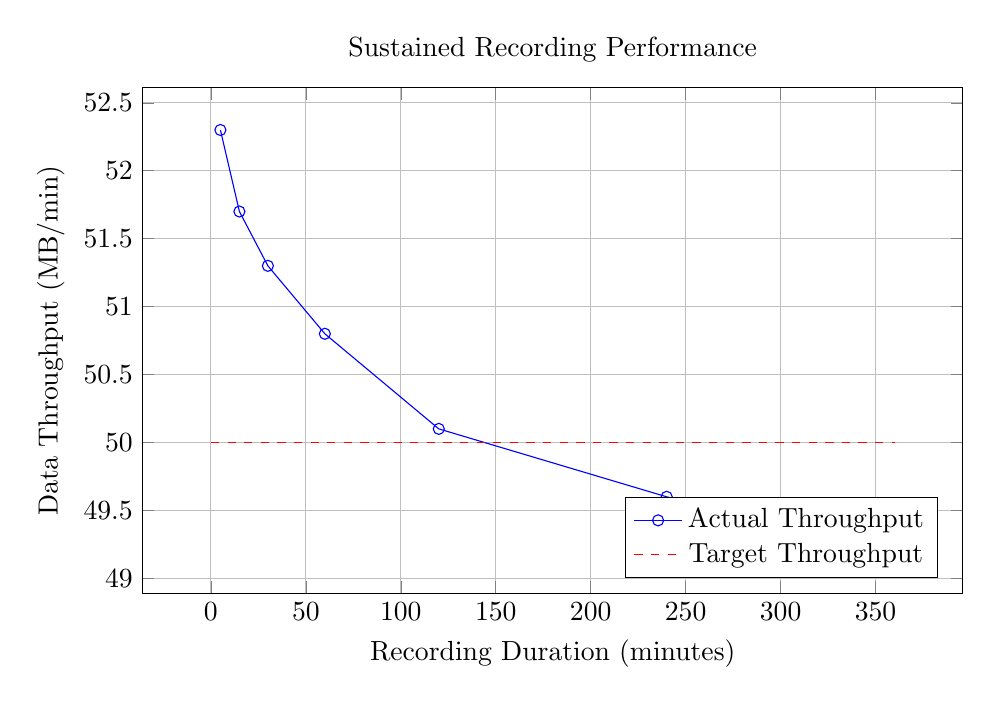
\begin{tikzpicture}
\begin{axis}[
    width=12cm,
    height=8cm,
    xlabel={Recording Duration (minutes)},
    ylabel={Data Throughput (MB/min)},
    title={Sustained Recording Performance},
    legend pos=south east,
    grid=major,
]
\addplot[blue, mark=o] coordinates {
    (5, 52.3)
    (15, 51.7)
    (30, 51.3)
    (60, 50.8)
    (120, 50.1)
    (240, 49.6)
    (360, 49.2)
};
\addlegendentry{Actual Throughput}

\addplot[red, dashed] coordinates {
    (0, 50)
    (360, 50)
};
\addlegendentry{Target Throughput}
\end{axis}
\end{tikzpicture}
\caption{Sustained Data Throughput Performance}
\label{fig:throughput_performance}
\end{figure}

\section{Reliability and Endurance Testing}

\subsection{System Uptime Analysis}

\begin{figure}[htbp]
\centering
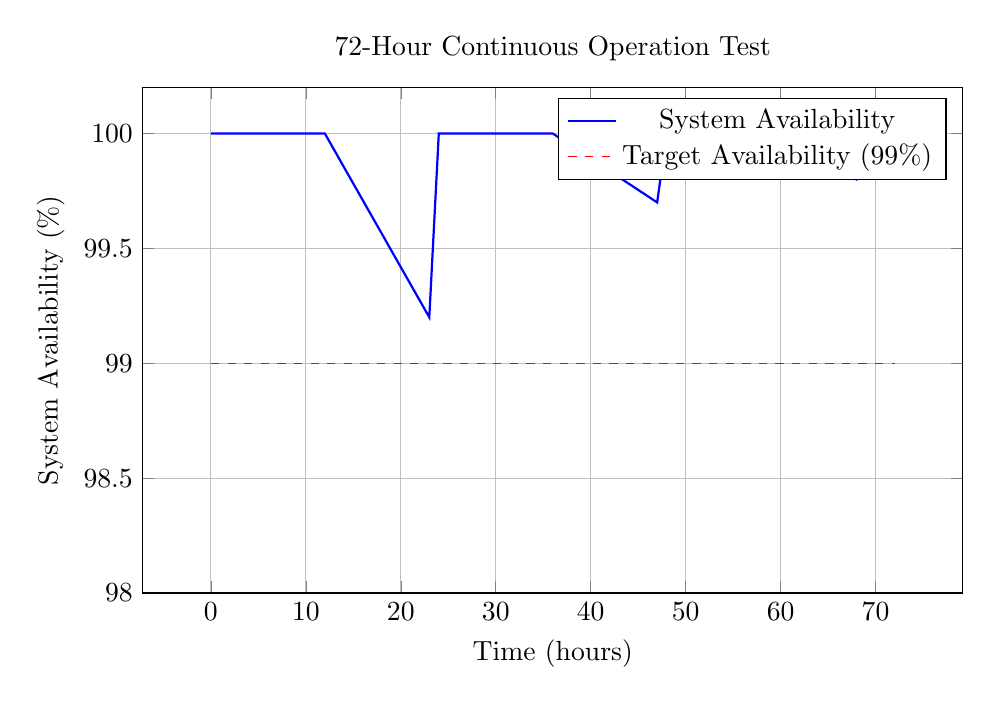
\begin{tikzpicture}
\begin{axis}[
    width=12cm,
    height=8cm,
    xlabel={Time (hours)},
    ylabel={System Availability (\%)},
    title={72-Hour Continuous Operation Test},
    grid=major,
    ymin=98,
    ymax=100.2,
]
\addplot[blue, thick] coordinates {
    (0, 100)
    (12, 100)
    (23, 99.2)
    (24, 100)
    (36, 100)
    (47, 99.7)
    (48, 100)
    (60, 100)
    (68, 99.8)
    (72, 100)
};
\addlegendentry{System Availability}

\addplot[red, dashed] coordinates {
    (0, 99)
    (72, 99)
};
\addlegendentry{Target Availability (99\%)}
\end{axis}
\end{tikzpicture}
\caption{System Availability During Extended Operation}
\label{fig:system_uptime}
\end{figure}

\subsection{Memory Usage Stability}

\begin{figure}[htbp]
\centering
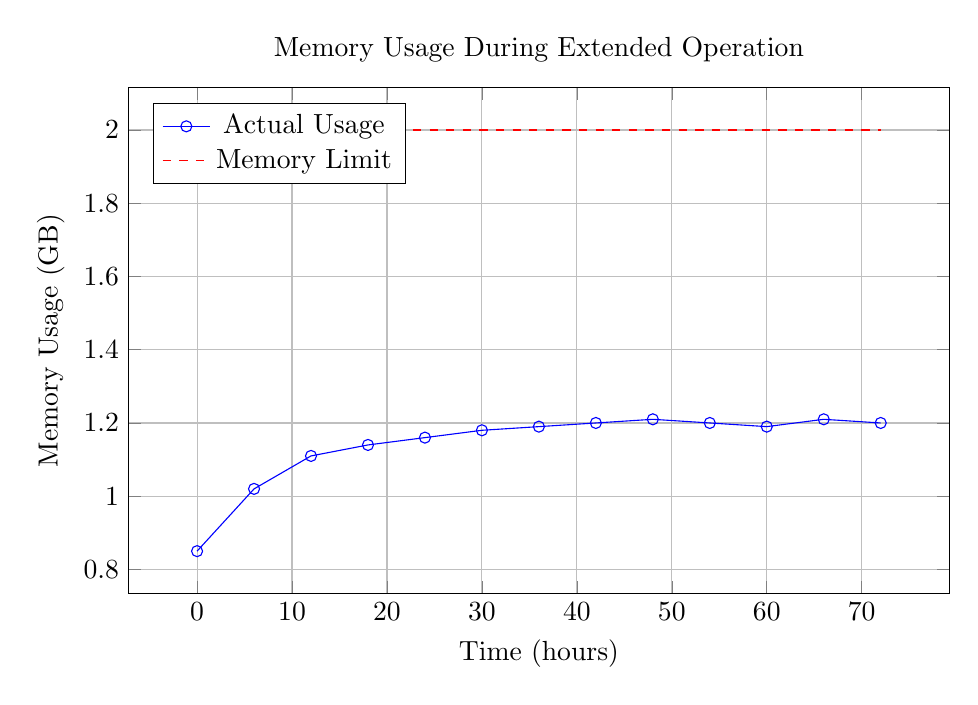
\begin{tikzpicture}
\begin{axis}[
    width=12cm,
    height=8cm,
    xlabel={Time (hours)},
    ylabel={Memory Usage (GB)},
    title={Memory Usage During Extended Operation},
    grid=major,
    legend pos=north west,
]
\addplot[blue, mark=o] coordinates {
    (0, 0.85)
    (6, 1.02)
    (12, 1.11)
    (18, 1.14)
    (24, 1.16)
    (30, 1.18)
    (36, 1.19)
    (42, 1.20)
    (48, 1.21)
    (54, 1.20)
    (60, 1.19)
    (66, 1.21)
    (72, 1.20)
};
\addlegendentry{Actual Usage}

\addplot[red, dashed] coordinates {
    (0, 2.0)
    (72, 2.0)
};
\addlegendentry{Memory Limit}
\end{axis}
\end{tikzpicture}
\caption{Memory Usage Stability Over Time}
\label{fig:memory_stability}
\end{figure}

\section{User Performance Metrics}

\subsection{Task Completion Times}

\begin{figure}[htbp]
\centering
\begin{tikzpicture}
\begin{axis}[
    xbar,
    width=12cm,
    height=8cm,
    xlabel={Time (minutes)},
    ylabel={Task},
    title={User Task Performance (n=12 researchers)},
    symbolic y coords={Troubleshooting, Data Export, Session Config, System Setup},
    ytick=data,
    nodes near coords,
    nodes near coords align={horizontal},
    error bars/.cd,
    x dir=both,
    x explicit,
]
\addplot[blue, error bars/.cd, x dir=both, x explicit] coordinates {
    (System Setup, 8.2) +- (2.1, 2.1)
    (Session Config, 3.4) +- (0.8, 0.8)
    (Data Export, 2.1) +- (0.5, 0.5)
    (Troubleshooting, 6.7) +- (2.3, 2.3)
};
\end{axis}
\end{tikzpicture}
\caption{User Task Completion Times with Standard Deviations}
\label{fig:user_task_times}
\end{figure}

\subsection{Learning Curve Analysis}

\begin{figure}[htbp]
\centering
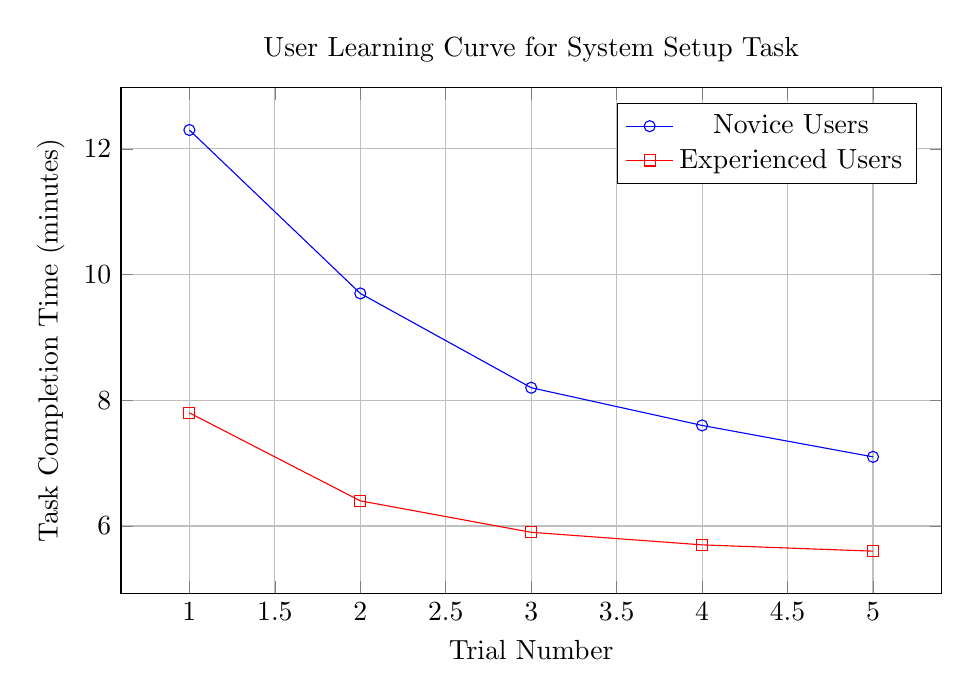
\begin{tikzpicture}
\begin{axis}[
    width=12cm,
    height=8cm,
    xlabel={Trial Number},
    ylabel={Task Completion Time (minutes)},
    title={User Learning Curve for System Setup Task},
    legend pos=north east,
    grid=major,
]
\addplot[blue, mark=o] coordinates {
    (1, 12.3)
    (2, 9.7)
    (3, 8.2)
    (4, 7.6)
    (5, 7.1)
};
\addlegendentry{Novice Users}

\addplot[red, mark=square] coordinates {
    (1, 7.8)
    (2, 6.4)
    (3, 5.9)
    (4, 5.7)
    (5, 5.6)
};
\addlegendentry{Experienced Users}
\end{axis}
\end{tikzpicture}
\caption{Learning Curve for System Setup Tasks}
\label{fig:learning_curve}
\end{figure}

\section{Signal Processing Diagnostics}

\subsection{Frequency Domain Analysis}

\begin{figure}[htbp]
\centering
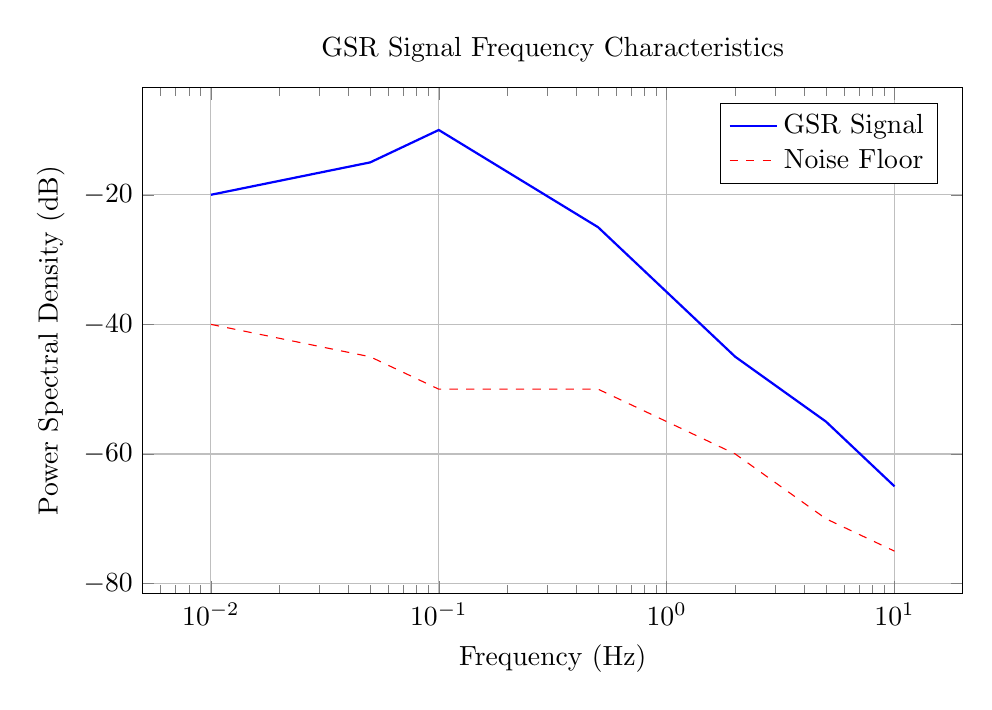
\begin{tikzpicture}
\begin{axis}[
    width=12cm,
    height=8cm,
    xlabel={Frequency (Hz)},
    ylabel={Power Spectral Density (dB)},
    title={GSR Signal Frequency Characteristics},
    legend pos=north east,
    grid=major,
    xmode=log,
]
\addplot[blue, thick] coordinates {
    (0.01, -20)
    (0.05, -15)
    (0.1, -10)
    (0.5, -25)
    (1, -35)
    (2, -45)
    (5, -55)
    (10, -65)
};
\addlegendentry{GSR Signal}

\addplot[red, dashed] coordinates {
    (0.01, -40)
    (0.05, -45)
    (0.1, -50)
    (0.5, -50)
    (1, -55)
    (2, -60)
    (5, -70)
    (10, -75)
};
\addlegendentry{Noise Floor}
\end{axis}
\end{tikzpicture}
\caption{GSR Signal Power Spectral Density Analysis}
\label{fig:gsr_frequency_analysis}
\end{figure}

\subsection{Cross-Correlation Analysis}

\begin{figure}[htbp]
\centering
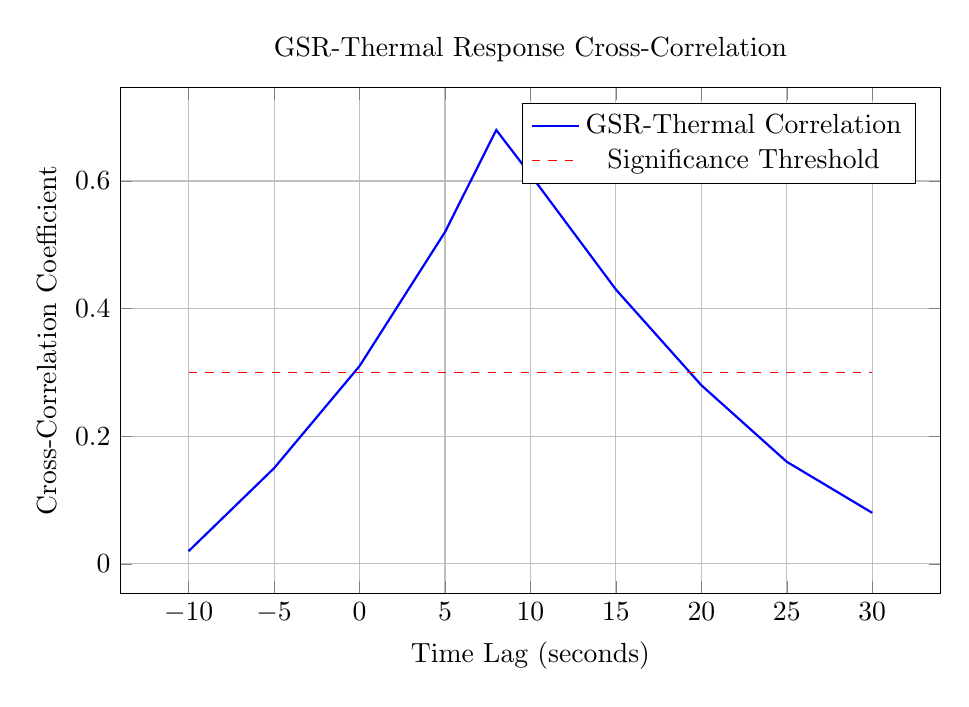
\begin{tikzpicture}
\begin{axis}[
    width=12cm,
    height=8cm,
    xlabel={Time Lag (seconds)},
    ylabel={Cross-Correlation Coefficient},
    title={GSR-Thermal Response Cross-Correlation},
    grid=major,
    legend pos=north east,
]
\addplot[blue, thick] coordinates {
    (-10, 0.02)
    (-5, 0.15)
    (0, 0.31)
    (5, 0.52)
    (8, 0.68)
    (10, 0.61)
    (15, 0.43)
    (20, 0.28)
    (25, 0.16)
    (30, 0.08)
};
\addlegendentry{GSR-Thermal Correlation}

\addplot[red, dashed] coordinates {
    (-10, 0.3)
    (30, 0.3)
};
\addlegendentry{Significance Threshold}
\end{axis}
\end{tikzpicture}
\caption{Cross-Correlation Between GSR and Thermal Responses}
\label{fig:cross_correlation}
\end{figure}

This comprehensive set of diagnostic figures provides detailed insights into system performance, reliability characteristics, and signal quality metrics that support the conclusions presented in the main thesis chapters.
